%!TEX root = thesis.tex
\chapter{Cross-Plane Thermal Transport in Superlattices}
\label{chap:slxp}
\section{Introduction}\blfootnote{Portions of this chapter have originally been published in \cite{ownSLXP} "Cross-plane Thermal Conduction in Superlattices: Impact of Multiple Length Scales on Phonon Transport" (2019), \textit{Journal of Applied Physics}, Vol. 125 (044304). Reproduced with permission from AIP Publishing.} 
A superlattice is a periodic structure of layers of two (or more) materials. Typically, the thickness of one layer is in the order of nanometers \cite{RN999}. Semiconductor superlattices are central to optoelectronic devices \cite{RN1000,Faist553,book_rogalski_infrared} including photodetectors, quantum cascade lasers and modulators. From the point of view of  thermal transport phenomena in nanoscale semiconductor superlattices, the changes in their properties arise from altered phonon transport dynamics, which can be broadly categorized into coherent and incoherent phonon effects. The term coherent refers to the underlying requirement of phase-preservation between phonons incident on and reflected from an interface between two materials. This condition for coherency, if satisfied across multiple interfaces, can manifest itself in a number of novel modifications of phonon dispersion relations including zone-folding effects, edge-flattening, and opening of thermal bandgaps under certain conditions of periodicity, wavelength, and phonon mean-free-paths \cite{RN362,RN132,RN253,RN394,RN329,RN399,RN393}. On the other hand, incoherent phonon effects result in a modified thermal transport dynamics due to reduced mean-free-paths or deviation in populations from Bose-Einstein distribution of phonons because of phonon-boundary scattering events (see \Cref{chap:predictive,chap:nt}, for example). Although both phonon dynamics (coherent and incoherent) arise from fundamentally different phenomena (i.e., phase preservation and diffuse scattering, respectively), they are controlled by the interaction of phonons with interfaces. This strong underlying connection of nanostructure surfaces to thermal transport coupled with (a) the existence of multiple interfaces and (b) a periodical pattern of these interfaces makes semiconductor superlattices a perfect choice for understanding heat conduction. 

The phenomenon of thermal phonon conduction in any periodic structure, including superlattices, is dependent on multiple key length scales [\Cref{fig:sl_schematic}] which are (i) the total size of the structure \gls{slsize}, (ii) the periodicity of the  structure \gls{period}, and (iii) interface surface properties, i.e., roughness \gls{eta} and correlation length \gls{cl}. In addition, the phonon length variables (iv) mean-free-path \gls{mfp} and (v) wavelength \gls{wl} are integral to the conduction phenomenon. A complex interplay between effects occurring at these various length scales coupled with the broadband nature of phonons determines the overall transport of heat in nanostructures. 
%Fig Schematic
\begin{figure}%[hbt!]	
	{\centering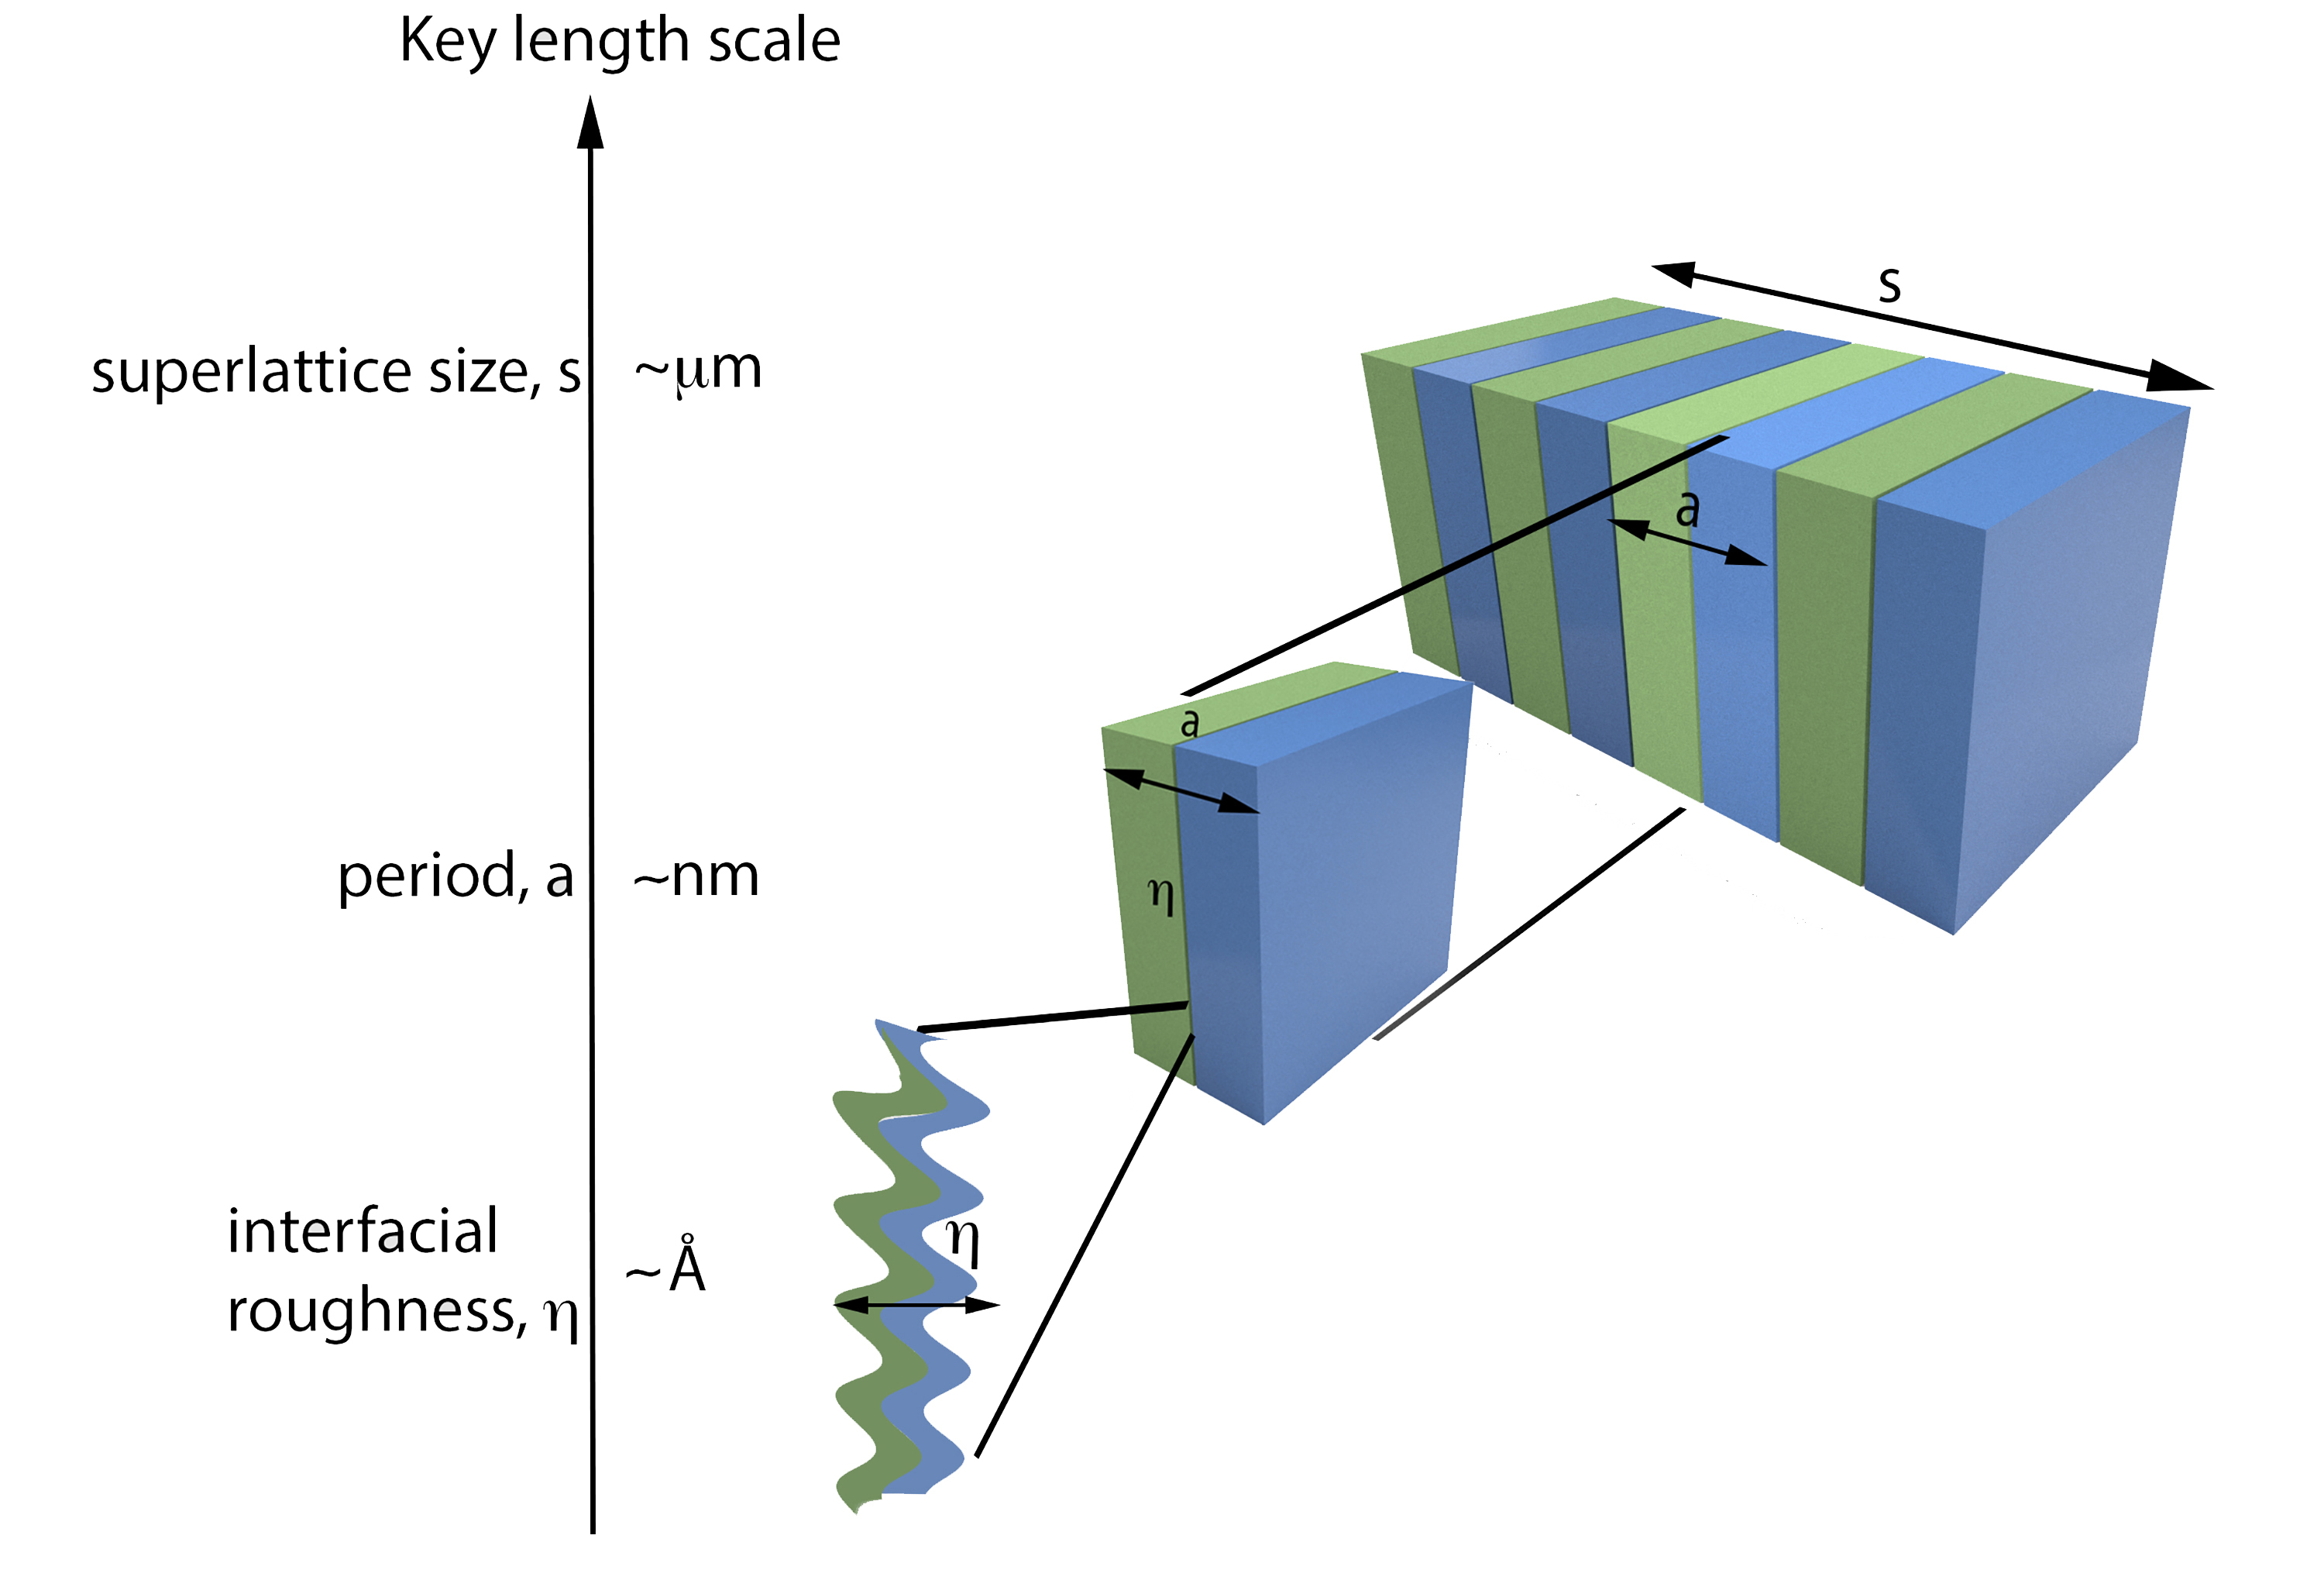
\includegraphics[width=0.93\textwidth]{/ch6/schematic.jpg}}
	\caption{Schematic showing key multiple length scales that control thermal conduction in superlattice structures. Thermal phonons scatter at rough interfaces ($\sim$\angstrom) between each layer within a unit cell of period \gls{period} ($\sim$nm) which combine to create a periodic superlattice nanostructure of total size \gls{slsize} ($\sim$\si{\micro}m).}
	\label{fig:sl_schematic}
\end{figure}

Despite several works over the last few decades, a clear understanding of the role of these fundamental length scales in phonon transport in superlattices remains lacking. For instance, a transition from coherent to incoherent thermal transport effects is expected in smooth-surface superlattices with increasing period length \gls{period}. The transition manifested as minima in thermal conductivity as a function of period has been shown in a few specific materials to date \cite{RN393,RN551}, indicating a need for an in-depth understanding of thermal transport in these structures. In addition to multiple reflections, the layered arrangement in a superlattice also creates an anisotropy in the structure that differentiates between heat flow parallel (in-plane) or perpendicular (cross-plane) to the interfaces, making them useful as directional heat spreaders for electronics \cite{RN545}. %

\section{Literature Overview of Si/Ge Superlattices}
Silicon and germanium are two popular and important semiconductors of commercial importance, and superlattices composed of these elements had attracted significant attention in experimental works. The work by Lee \etal \cite{RN282}, Borca-Tasciuc \etal \cite{RN298}, and Huxtable \etal \cite{RN361,RN297}, remains the primary source of experimental data for the cross-plane thermal conductivities in Si/Ge superlattices. All of these works alluded to the importance of the interface quality and defect density -- features which are still poorly quantified and understood-- in their thermal conductivity measurements. As noted in a recent study \cite{RN544}, the absence of consistency among the measured thermal conductivities in many of these studies \cite{RN282,RN298,RN300}, leaves a gaping hole in our understanding of thermal transport in these superlattices. From a theoretical standpoint, numerous techniques have been developed to understand thermal transport in superlattices \cite{RN266,RN264,RN305,RN306,RN357,RN353} but quantitative predictions of thermal transport properties in realistic nanostructures, accounting for interfacial scattering and phonon-phonon scattering across all temperatures, continue to be an open challenge. A quick glimpse at the literature reveals the underlying dissonance in the predictions by theoretical models. For instance, first-principle calculations and the Boltzmann transport equation (BTE) showed that interfacial roughness serves to reduce the thermal conductivity in Si/Ge superlattices \cite{RN328,RN294,RN169}. In contrast, Green function calculations predicted that lattice thermal conductivity of Si/Ge superlattices with rough interfaces could be higher than those with smooth interfaces if the number of periods were small \cite{RN295}. Furthermore, molecular dynamics \cite{RN319,RN353,RN262} have noted that the absence of a coherent transport signature (i.e., thermal conductivity minimum with period length) could be explained by the interfacial roughness in Si/Ge superlattices. First-principle approaches, on the other hand, showed that even after inclusion of interfacial disorder as perturbations, minima in thermal conductivity could still be observed \cite{RN262}. Thus, there is a clear need for a detailed study of cross-plane thermal transport in Si/Ge superlattices, addressing the role of interfaces and impact of all other relevant length variables on thermal conductivity, i.e., the periodicity \gls{period}, the mean-free-path of phonons \gls{mfp}, wavelength of phonons \gls{wl}, and total size/thickness of the structure \gls{slsize}.
\par Theoretical approaches based on the phonon Boltzmann transport equation (BTE) hold an untapped potential in being able to effectively connect theoretical predictions with experiments. The flexibility of BTE approaches allows for treatment of heat transport in various geometrical domains without relying on limiting assumptions about surface properties. Historically, BTE based approaches considered the use of fitting specularity parameters that limited the physical insights. However, as we discussed in \Cref{chap:predictive}, it is possible to incorporate rigorous surface description within the Boltzmann framework, which can be used to provide quantitative predictions on thermal transport. Moreover, using first-principle calculations to yield material-specific phonon properties as inputs to BTE can create accurate, computationally cost efficient, and comprehensive predictive models for experimental nanostructures provided that the treatment of phonon-interface behavior can be rigorously included. Specifically, for superlattices, the radiative/intensity form of BTE for superlattices \cite{RN267,RN348} dealing with an overall scalar intensity of phonons rather than with individual mode dependent populations precludes the inclusion of incident angle dependent interface-phonon scattering. Recently, solutions to BTE based on the treatment of boundary scattering without transmission between different layers have been developed \cite{RN328,RN372}. Rigorous solutions to the BTE with detailed boundary conditions to obtain local mode dependent phonon populations have been applied to heat transport problems in thin-films, nanowires, (see \Cref{chap:predictive,chap:diff_boundary}) and recently to in-plane thermal transport in layered nanomaterials \cite{RN396} (also see \Cref{chap:layered}). However, such a rigorous approach dealing with mode-by-mode calculation of phonon populations while accounting for interfacial surface characteristics, incident phonon properties, and phonon coupling is currently absent for cross-plane thermal transport in superlattices.
\section{Methodology}
The methodology is based on the layered nanomaterials solution discussed in \Cref{chap:layered}. The general first-order solution to the phonon Boltzmann transport equation under a small temperature gradient in the \textit{cross-plane} $x$ direction, can be written as \cite{ownSLXP},
\begin{equation} 
  g_i^\pm=  -v_{i|x} \tau_{i}\frac{\partial T}{\partial x}\frac{\partial f_{i}^{BE}}{\partial T}\Bigg(1+\Phi_{i}^\pm\exp\Big(-\dfrac{x}{\tau_{i} v_{i|x}}\Big) \Bigg)
\label{eq:ch6-gpm}
\end{equation}
Despite the similarity to \Cref{eq:ch5-gpm}, here the dependence of deviation function $g^\pm$ is independent of the z-dimension. We note that the deviation function depends on the direction of phonon propagation indicated by + and - symbols for propagation along the applied thermal gradient and opposite to the applied thermal gradient, respectively. Since the superlattice is comprised of periodically repeating unit cell, an interfacial phonon balance at the unit cell interface \cite{RN396} along with an anti-symmetric deviation from equilibrium for phonons moving in opposite directions in the superlattice \cite{RN582} are sufficient conditions to solve for deviation functions in the cross-plane direction. Individual layers thermal conductivities are obtained using \Cref{eq:pop_fourier}. The overall cross-plane thermal conductivity of the superlattice structure is evaluated by considering flux conservation in the direction of the thermal gradient. Due to the presence of interfaces between the two materials in adjoining layers of the superlattice, the temperature gradient across the interfaces would change abruptly, which is accounted for using the thermal boundary resistance ($R_\textrm{TBR}$) \cite{RN328}. Thus, the cross-plane thermal conductivity $\kappa_\textrm{cp}$ of the superlattice can be expressed as,
\begin{equation} 
\dfrac{t_1+t_2}{\kappa_\textrm{cp}}=\dfrac{t_1}{\kappa_1}+\dfrac{t_2}{\kappa_2}+R_\textrm{TBR}
\end{equation}
where $t_1$ and $t_2$ are, respectively, the thicknesses of the two constitutive layers of the superlattice and $\kappa_1$ and $\kappa_2$ are the individual thermal conductivities of the layers.
\section{Key Results and Discussion}
%Figure2
We first predict the thermal conductivity of Si/Ge superlattices at room temperature (\gls{T} = 300 K) in \Cref{fig:ch6-2}(a) and low temperature (\gls{T} = 80 K) in \Cref{fig:ch6-2}(b). We show how the thermal conductivity increases with increasing period thicknesses for different superlattice interface conditions ranging from very smooth to very rough surfaces. The increasing period thickness a reduces the interface density and allows phonons to travel longer distances between scatterings from interfaces. The reduction in interface density thus directly translates to increased phonon mean-free-paths and thermal conductivities. Interestingly, we observe that even at large period thicknesses (\gls{period} $\sim$ 5 \si{\micro}m), the thermal conductivity is below the value in the absence of phonon-surface scattering (i.e., bulk value), indicating the wide spectrum of phonon mean-free-paths and the strong interface scattering phenomenon in cross-plane phonon transport. The thermal conductivity predictions for different roughness values converge at larger period thicknesses owing to the reduced interface scattering events, removing the difference arising due to diffuse scattering. Interestingly, for small period \gls{period} $\sim$ 5 nm at low temperature \gls{T} = 80 K, introduction of a slight degree of disorder (\gls{eta} $\sim$ 0.05 nm) leads to a strong reduction in superlattice thermal conductivity. In this case, the small periodicity of the superlattice coupled with the reduced phonon-phonon scattering at low temperatures allows phonons to scatter strongly from the introduced disorder at the surfaces. Furthermore, it is observed that the increase of surface roughness from \gls{eta} = 0.5 nm to \gls{eta} = 1.0 nm leads to a minimal change in cross-plane thermal conductivity, indicating the onset of nearly complete diffusive scatterings at these roughnesses in these structures. We also plot in \Cref{fig:ch6-2} the experimentally measured thermal conductivities in Si/Ge superlattices and find excellent agreement despite the variability in the experimental data. We note that experimental growth of superlattices relies on the use of buffer layers as well as the use of surfactants whose presence in samples could influence the measured thermal conductivity \cite{RN361,RN297,RN298,RN300}. These experimental factors (e.g., the role of buffer layers, creation of native oxides, etc.) are not included in our model which is aimed at understanding the role of all length scales in thermal transport.
\begin{figure}[hbt]
  \centering 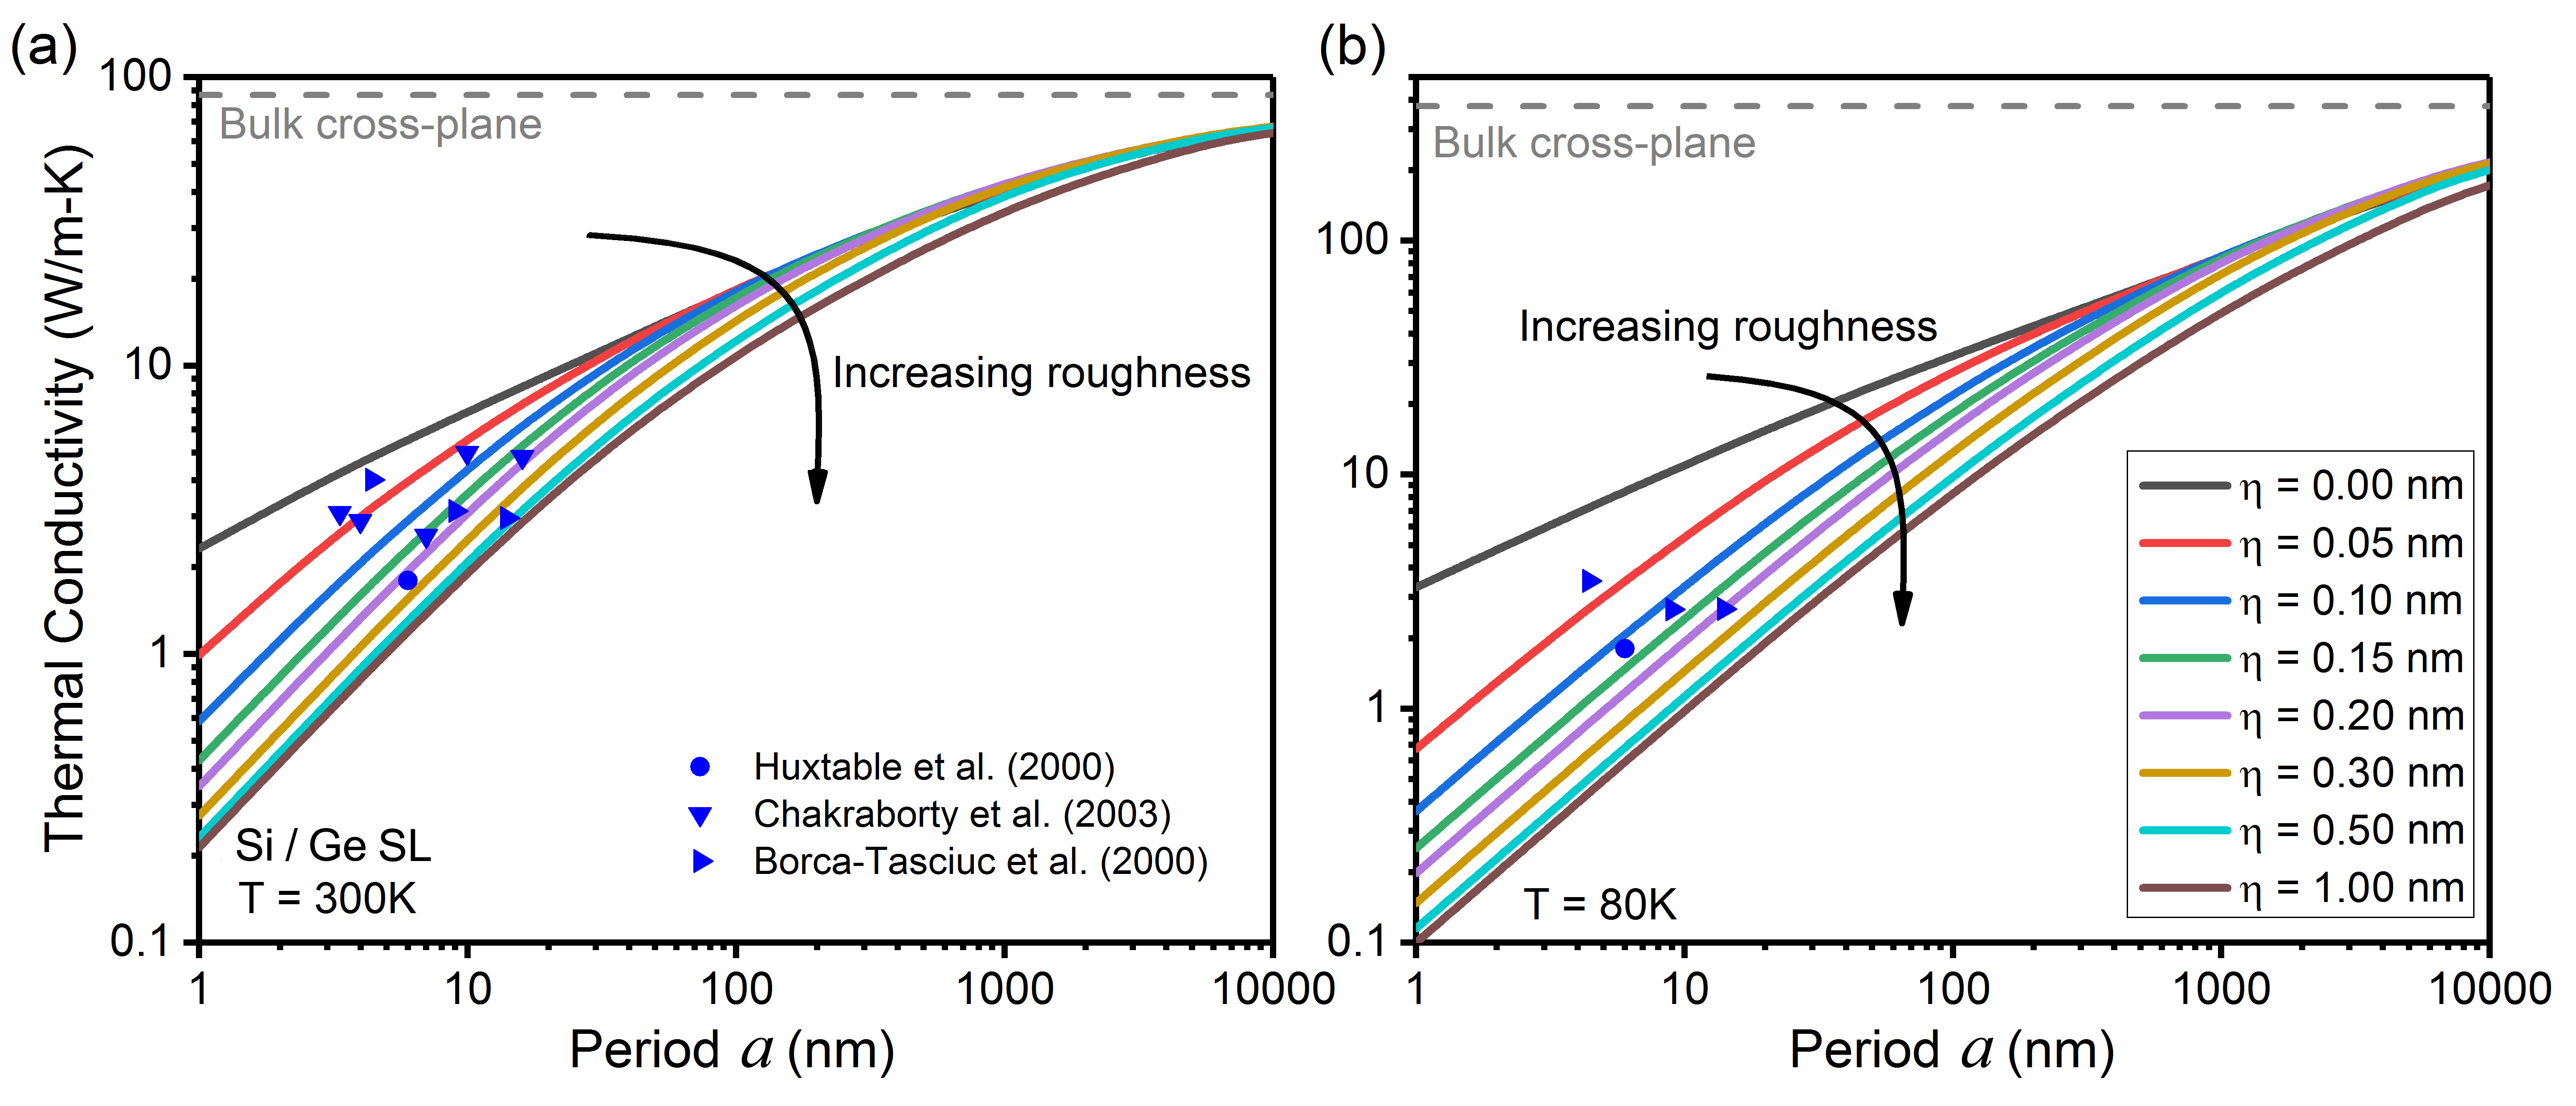
\includegraphics[width=1.0\textwidth]{figures/ch6/Fig2.jpg}
  \caption{Cross-plane thermal conductivity \gls{K} in Si/Ge superlattices at (a) \gls{T} = 300 K and (b) 80 K as a function of period thickness \gls{period}. \gls{K} predictions for different interfacial roughnesses \gls{eta} are shown and compared against available experimental data (scatter points).}
  \label{fig:ch6-2}
\end{figure}
%Figure3
Additionally, the large contrast in lattice constants between Si and Ge unit cells heightens the challenge of obtaining a control over interfacial roughness experimentally, which is a key factor in determining thermal transport in nanostructures \cite{RN396}. Note that our analysis is focused on phonon transport in the absence of coherent interference effects. It is expected that a high interfacial roughness in experimental Si/Ge superlattices prevents coherent effects from playing a dominant role \cite{RN544}. Our findings clearly show the importance of interface conditions, in particular for small period superlattices, as they can yield strong modulations in thermal transport, reinforcing the need for quantitative approaches to model and report superlattice surface conditions. In \Cref{fig:ch6-3}(a) and (b), we also compare our numerical predictions against experimental measurements on \sige{0.84}{0.16}/\sige{0.76}{0.24} alloy superlattices with equal volume fractions \cite{RN361}. We find excellent agreement with the experimental measurements and observe that the thermal conductivity has a very weak dependence on interfacial roughness in these superlattices. The weak dependence on interfacial scattering can be explained by the material similarity of the superlattice layers, which reduces the influence of roughness on phonon transmission at interfaces. For a different experimental data-set of Si/\sige{0.70}{0.30} superlattices with two-third of volume fraction comprised by the Si layer \cite{RN361}, we observe qualitative agreement with the data at \gls{T} = 300 K but we find that the reported thermal conductivities are larger than the numerical predictions. The dependence of thermal conductivity on surface roughness is observed to be stronger unlike the \sige{0.84}{0.16}/\sige{0.76}{0.24} case, since the materials across interfaces are more distinct. Thus, future experimental work with quantification of surface roughness especially in alloy superlattices would be an exciting avenue to experimentally validate the predictions of our model as well as advance the understanding of thermal transport in these nanostructures. Since surface roughness and correlation length are statistical quantities, techniques that can extract and combine surface profiles across the length of the interface are needed. Such techniques involving stitching of transmission electron microscope (TEM) images to extract surface profiles followed by background elimination \cite{RN131} have been used for nanowires while similar efforts for superlattices are currently lacking. 
\begin{figure}[hbtp]
  \centering 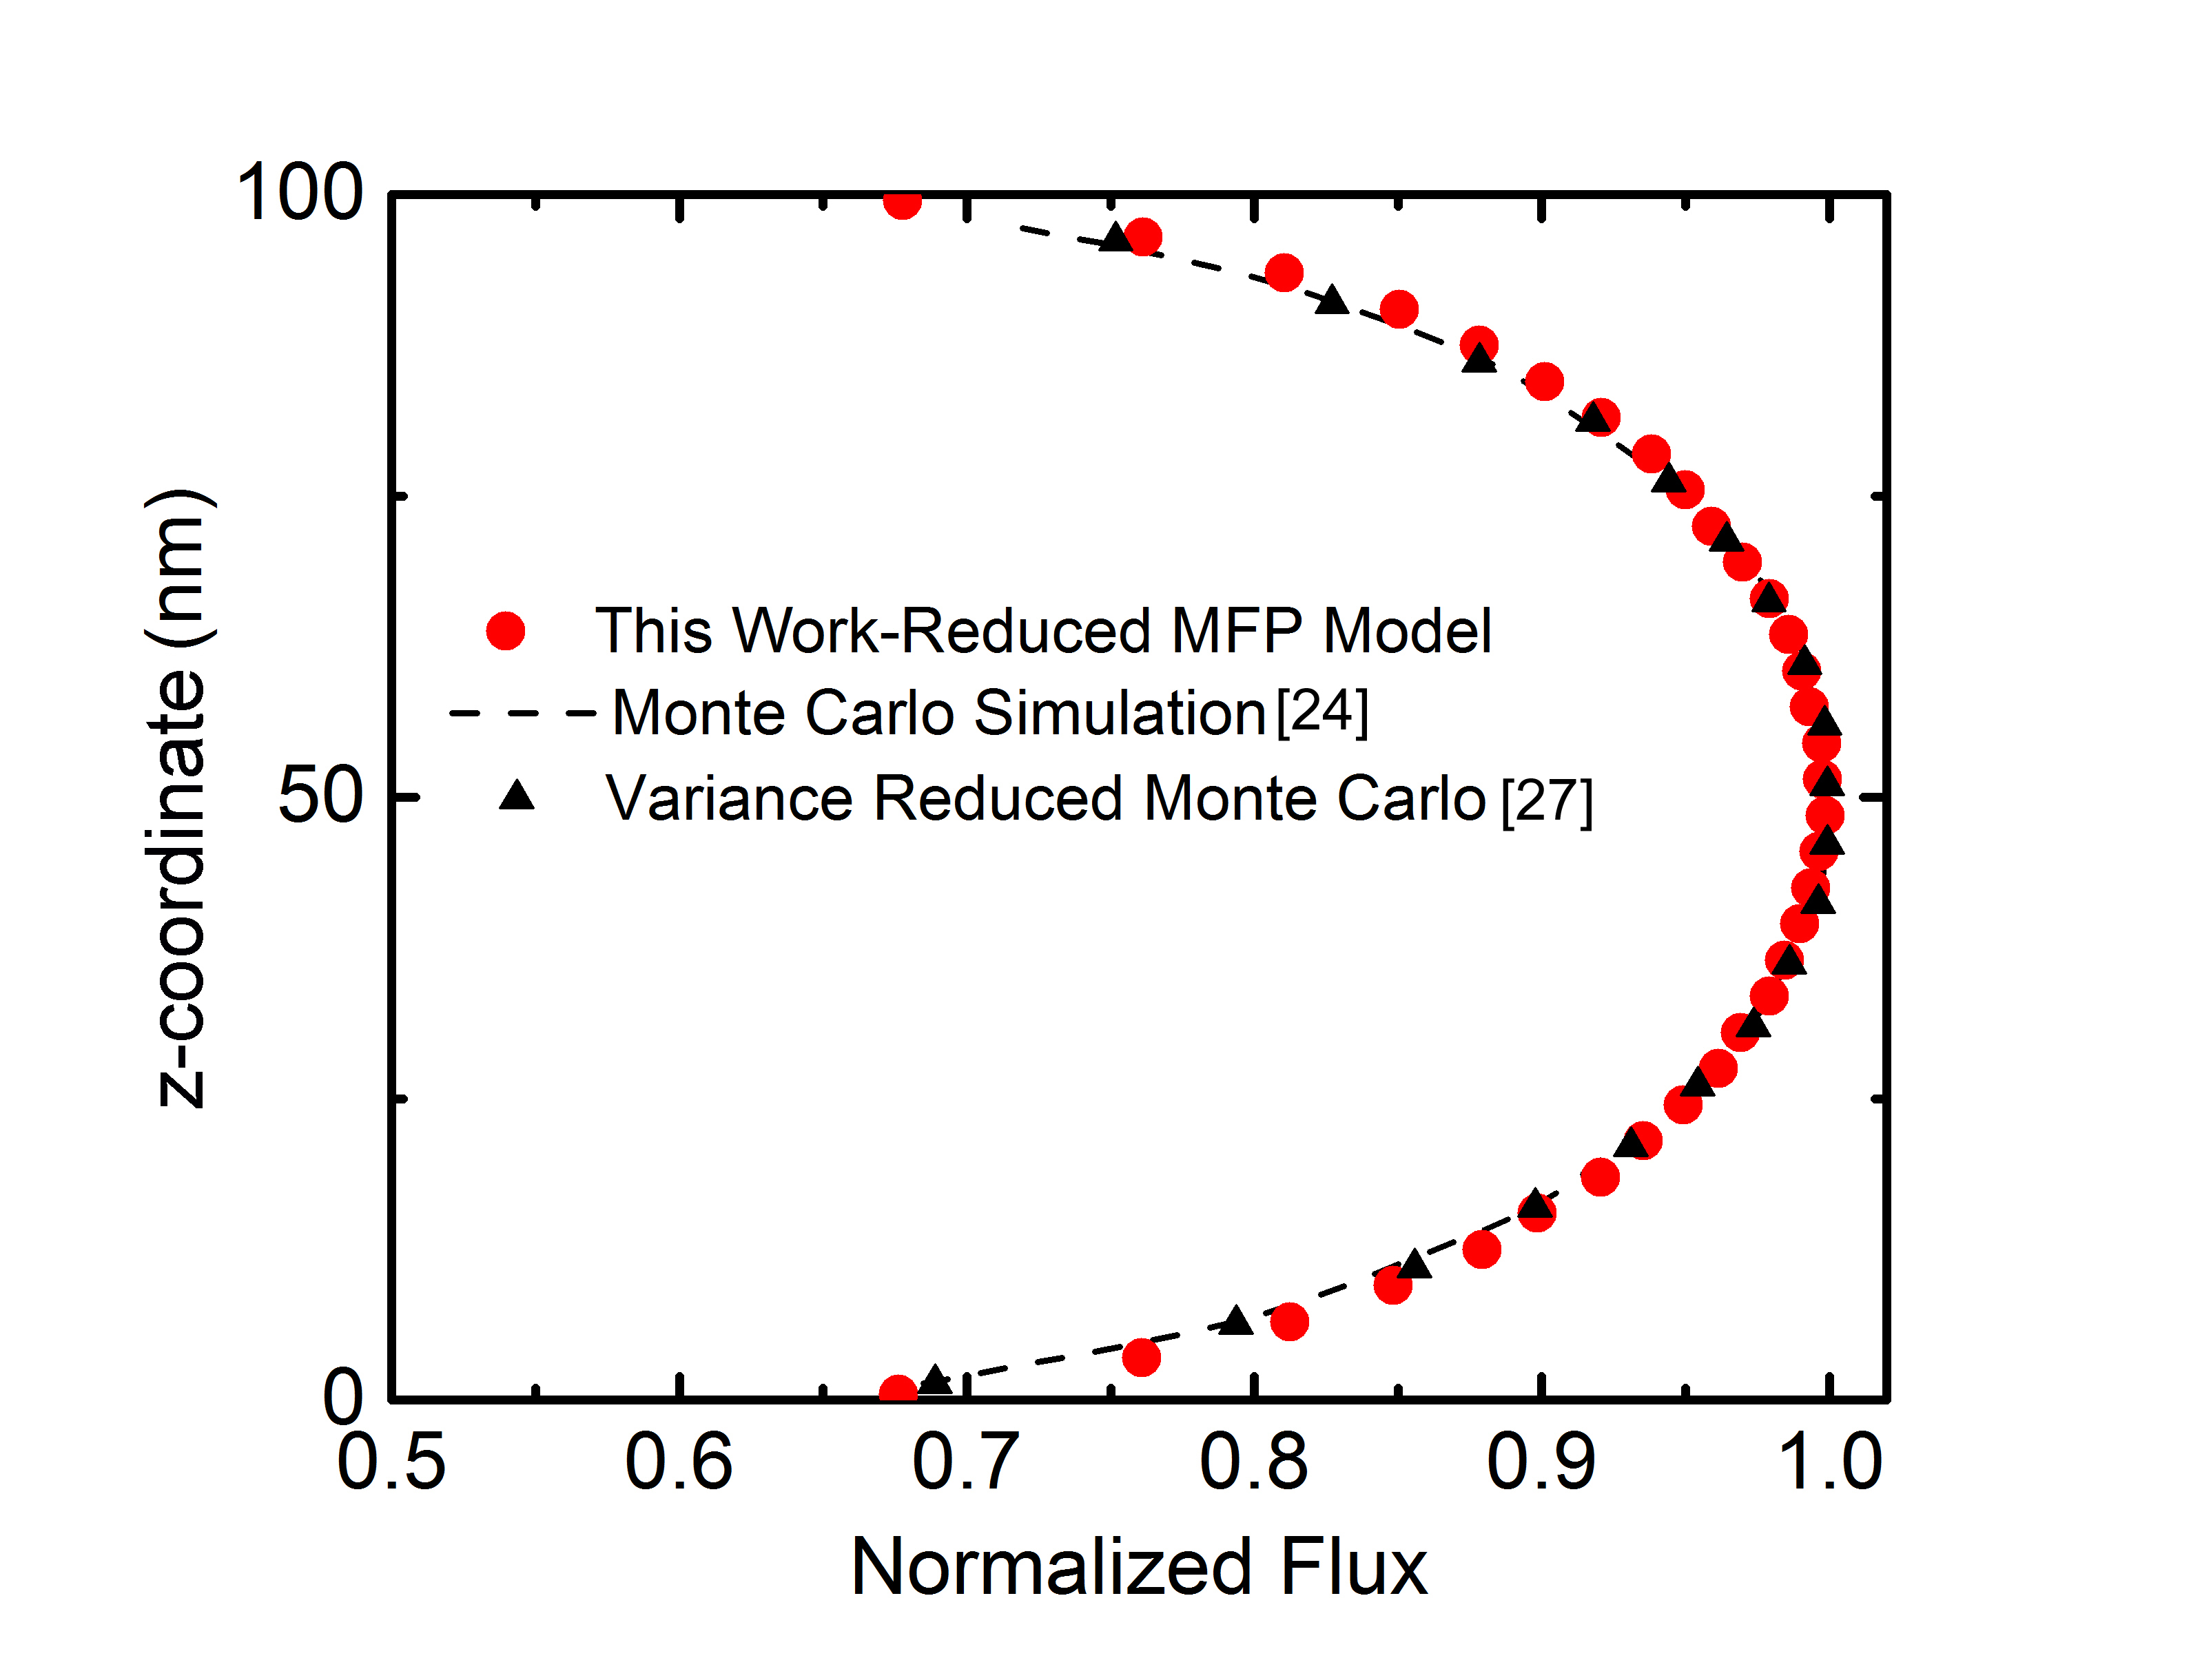
\includegraphics[width=1.0\textwidth]{figures/ch6/Fig3.jpg}
  \caption{Cross-plane thermal conductivity in experimental alloyed superlattices as a function of period, for different interfacial roughness values. Thermal conductivities are evaluated at \gls{T} = 300 K in [(a) and (c)] and 80 K in [(b) and (d)]. Panels (a) and (b) are for \sige{0.84}{0.16}/\sige{0.76}{0.24} superlattices and (c) and (d) are for Si/\sige{0.70}{0.30} superlattices.}
  \label{fig:ch6-3}
\end{figure}
%Figure4
\par Based on the large number of SiGe alloy superlattice experiments, an interesting question that has not been answered is the impact of alloying one layer vs both layers in the superlattice. To address this question, we consider three possible configurations of alloying, i.e., we alloy either one of the two layers of a Si/Ge superlattice, and also alloy both the layers, and compare all configurations against an unalloyed Si/Ge superlattice. We show in \Cref{fig:ch6-4} the corresponding numerical predictions for the thermal conductivities for different periods, temperatures, and interface conditions. We find that the thermal conductivity in all the superlattices increases with increasing period \gls{period}, irrespective of the inner surface condition, temperature, or alloying. These results are in agreement with an earlier report \cite{RN267} and can be understood by the increased effective mean-free-paths with increasing distance between the boundaries under incoherent transport. However, unlike the conclusions of this report, we find that the thermal boundary resistance does not play a determining role in our predictions. We note that it has also been reported \cite{RN291} that thermal transport in superlattices cannot be attributed solely to thermal boundary resistance. In our calculations, one order change in thermal boundary resistance (TBR) at room temperature from $3\times 10^{-9}$ \si{\meter\squared\per\kilo\watt}  \cite{RN358} (value used in this report) to $3\times 10^{-8}$ \si{\meter\squared\per\kilo\watt} leads to a negligible change in the thermal conductivity (\textless1\% at \gls{period} = 5 nm), quantifying the small impact TBR has on thermal conductivity value of the Si/Ge superlattices. This finding can be understood by an order of magnitude analysis on individual resistances of the Si and Ge layers, and the effects of TBR between the layers, which becomes small with increasing period. Interestingly, we observe that the alloying of either of the Si or Ge layers leads to a similar reduction in thermal conductivity (red and blue lines) for all periods and surface conditions. We note that alloying of either of the layers leads to impurity scattering for phonons in the alloyed layer and also for phonons that can couple across the interfaces and travel in both the materials. Since the conductivities of the layers are arranged in parallel, the thermal transport is critically determined by the thermal conductivity of the layer with smaller conductivity. Thus, we conclude that alloying either layer in a Si/Ge superlattice to a small degree leads to similar thermal conductivities. In the case when both the layers are alloyed, phonons in all the layers have reduced mean-free-paths due to scattering by alloy atoms, lowering the thermal transport further (brown lines). This behavior persists for both smooth (\gls{eta} = 0.1 nm) and rough (\gls{eta} = 0.5 nm) inner interfaces. We also observe that the thermal conductivity of unalloyed Si/Ge superlattices especially at low temperatures (e.g., \gls{T} = 80 K) with rough inner interface decreases linearly with decreasing periods for \gls{period} \textless 100 nm [\Cref{fig:ch6-4}(c)], indicative of nearly ballistic transport within the layers at these temperatures.
\begin{figure}[hbt]
  \centering 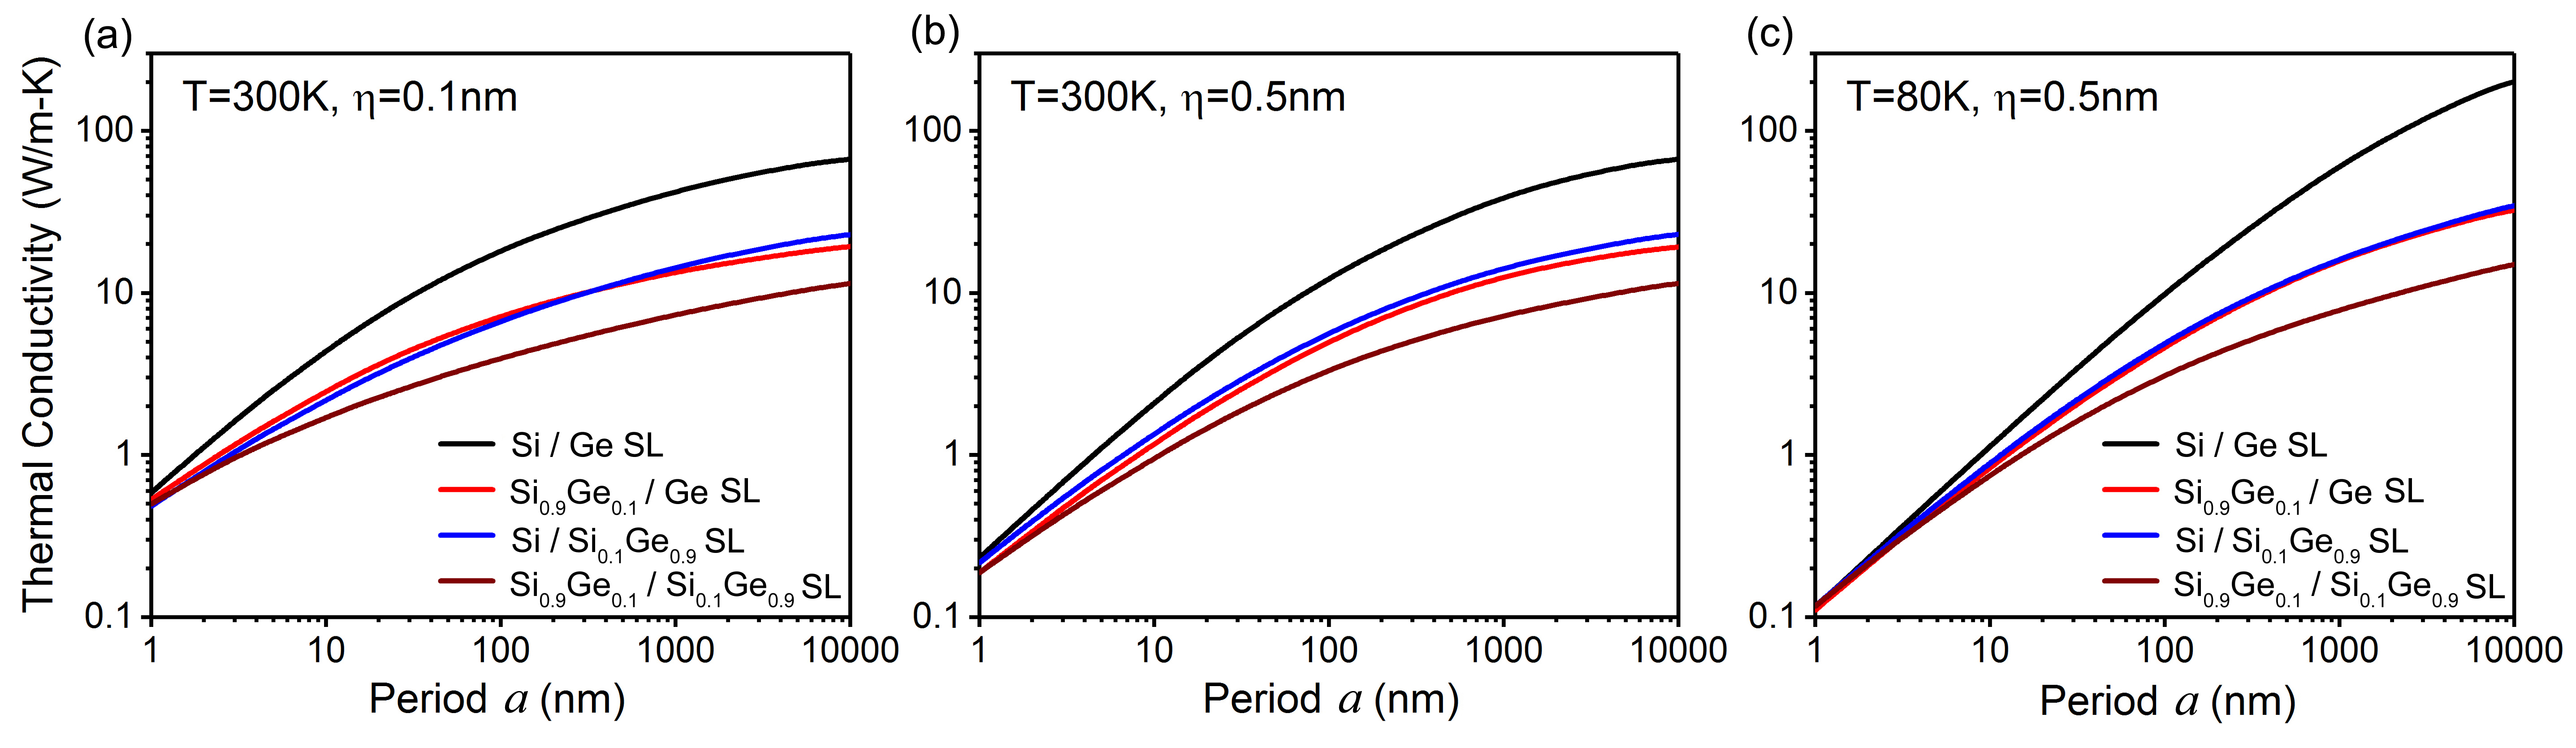
\includegraphics[width=1.0\textwidth]{figures/ch6/Fig4.jpg}
  \caption{Cross-plane thermal conductivity in Si/Ge (black lines), \sige{0.90}{0.10}/Ge (red lines), Si/\sige{0.10}{0.90} (blue lines), and \sige{0.90}{0.10}/\sige{0.10}{0.90} (brown lines) superlattices at (a) \gls{eta} = 0.1 nm and \gls{T} = 300 K, (b) \gls{eta} = 0.5 nm and \gls{T} = 300 K, and (c) \gls{eta} = 0.5 nm and \gls{T} = 80 K, as a function of period thickness \gls{period}.}
  \label{fig:ch6-4}
\end{figure}

%Figure5
\par Importantly, there is also the possibility of quasi-ballistic transport across the entire superlattice structure, which leads to another important length scale -- the total structure size \gls{slsize}. The existence of thermal conductivity that increases linearly with total structure size has been experimentally observed in GaAs superlattices \cite{RN394}, which has been corroborated by a recent study \cite{RN544}. To understand the role of structure size \gls{slsize} on thermal transport in Silicon-Germanium based superlattices, we next use our approach to predict the thermal conductivity in Si/Ge and \sige{0.90}{0.10}/\sige{0.10}{0.90} superlattices as a function of total size for different periods at \gls{T} = 300 K (\Cref{fig:ch6-5}). The finite size of the structure limits the number of periods that can exist in the structure. Strictly speaking, finite sized structures need to be modeled by applying phonon population balance at each surface (i.e. interfaces and boundaries). In our approach, we consider a unit cell of two layers as described in the Methodology and evaluate the thermal conductivity assuming a fully diffusive boundary after a specified number of periods. \Cref{fig:ch6-5} shows that the thermal conductivity of Si/Ge and SiGe alloyed superlattices is significantly influenced by the structure size \gls{slsize} (or number of periods, $N = s/a$), and thus these features need to be reported as well in experiments for consistent comparison between measurements. We observe that for small period superlattices at room temperature [\Cref{fig:ch6-5}(c,d)], a superlattice with smooth interface (solid lines) shows an increasing trend of thermal conductivity with increasing structure size, while for superlattices with rough interfaces (dashed lines), the total structure size change leads to a smaller increase in thermal conductivity. These findings indicate that smoother interfaces allow phonons to cross multiple periods and the total structure size \gls{slsize} becomes a limiting factor in their mean-free-paths. However, for alloyed superlattices [\Cref{fig:ch6-5}(b)], we observe that the structure size \gls{slsize} can influence the thermal conductivities of superlattices with both small and large roughness especially for period \gls{period} = 200 nm due to the existence of large mean-free-path phonons in large period superlattices. To further elucidate the thermal conductivity dependence on structure size in alloyed superlattices without having to consider the variability in individual period size \gls{period}, we added one period at a time in \Cref{fig:ch6-6}. The alloyed superlattice exhibits a significance dependence of \gls{K} on the number of periods, indicative of the large phonon mean-free-paths in these structures. We also find that the effect of adding periods leading to a quasi-linear increase in conductivity persists even at \gls{T} = 300 K highlighting the existence of phonons that can cross multiple interfaces at these temperatures provided the surface roughness is low. The impact of adding periods on conductivity is slightly stronger at \gls{T} = 80 K due to the diminishing phonon-phonon scattering at these temperatures. These results support the conclusion that phonons that can cross multiple interfaces are better observed at low temperatures and smooth interfaces, in agreement with the conclusions for GaAs/AlAs superlattices in Ref. \cite{RN394}. Since multiple interfacial scattering is a key criterion for interference phenomenon, it can be concluded that structures allowing for such large mean-free-path phonons to propagate (i.e., low temperatures and low roughness) would be better candidates to explore coherent interference modifications in thermal transport \cite{RN362,RN394,RN393}.
\begin{figure}[hbtp]
  \centering 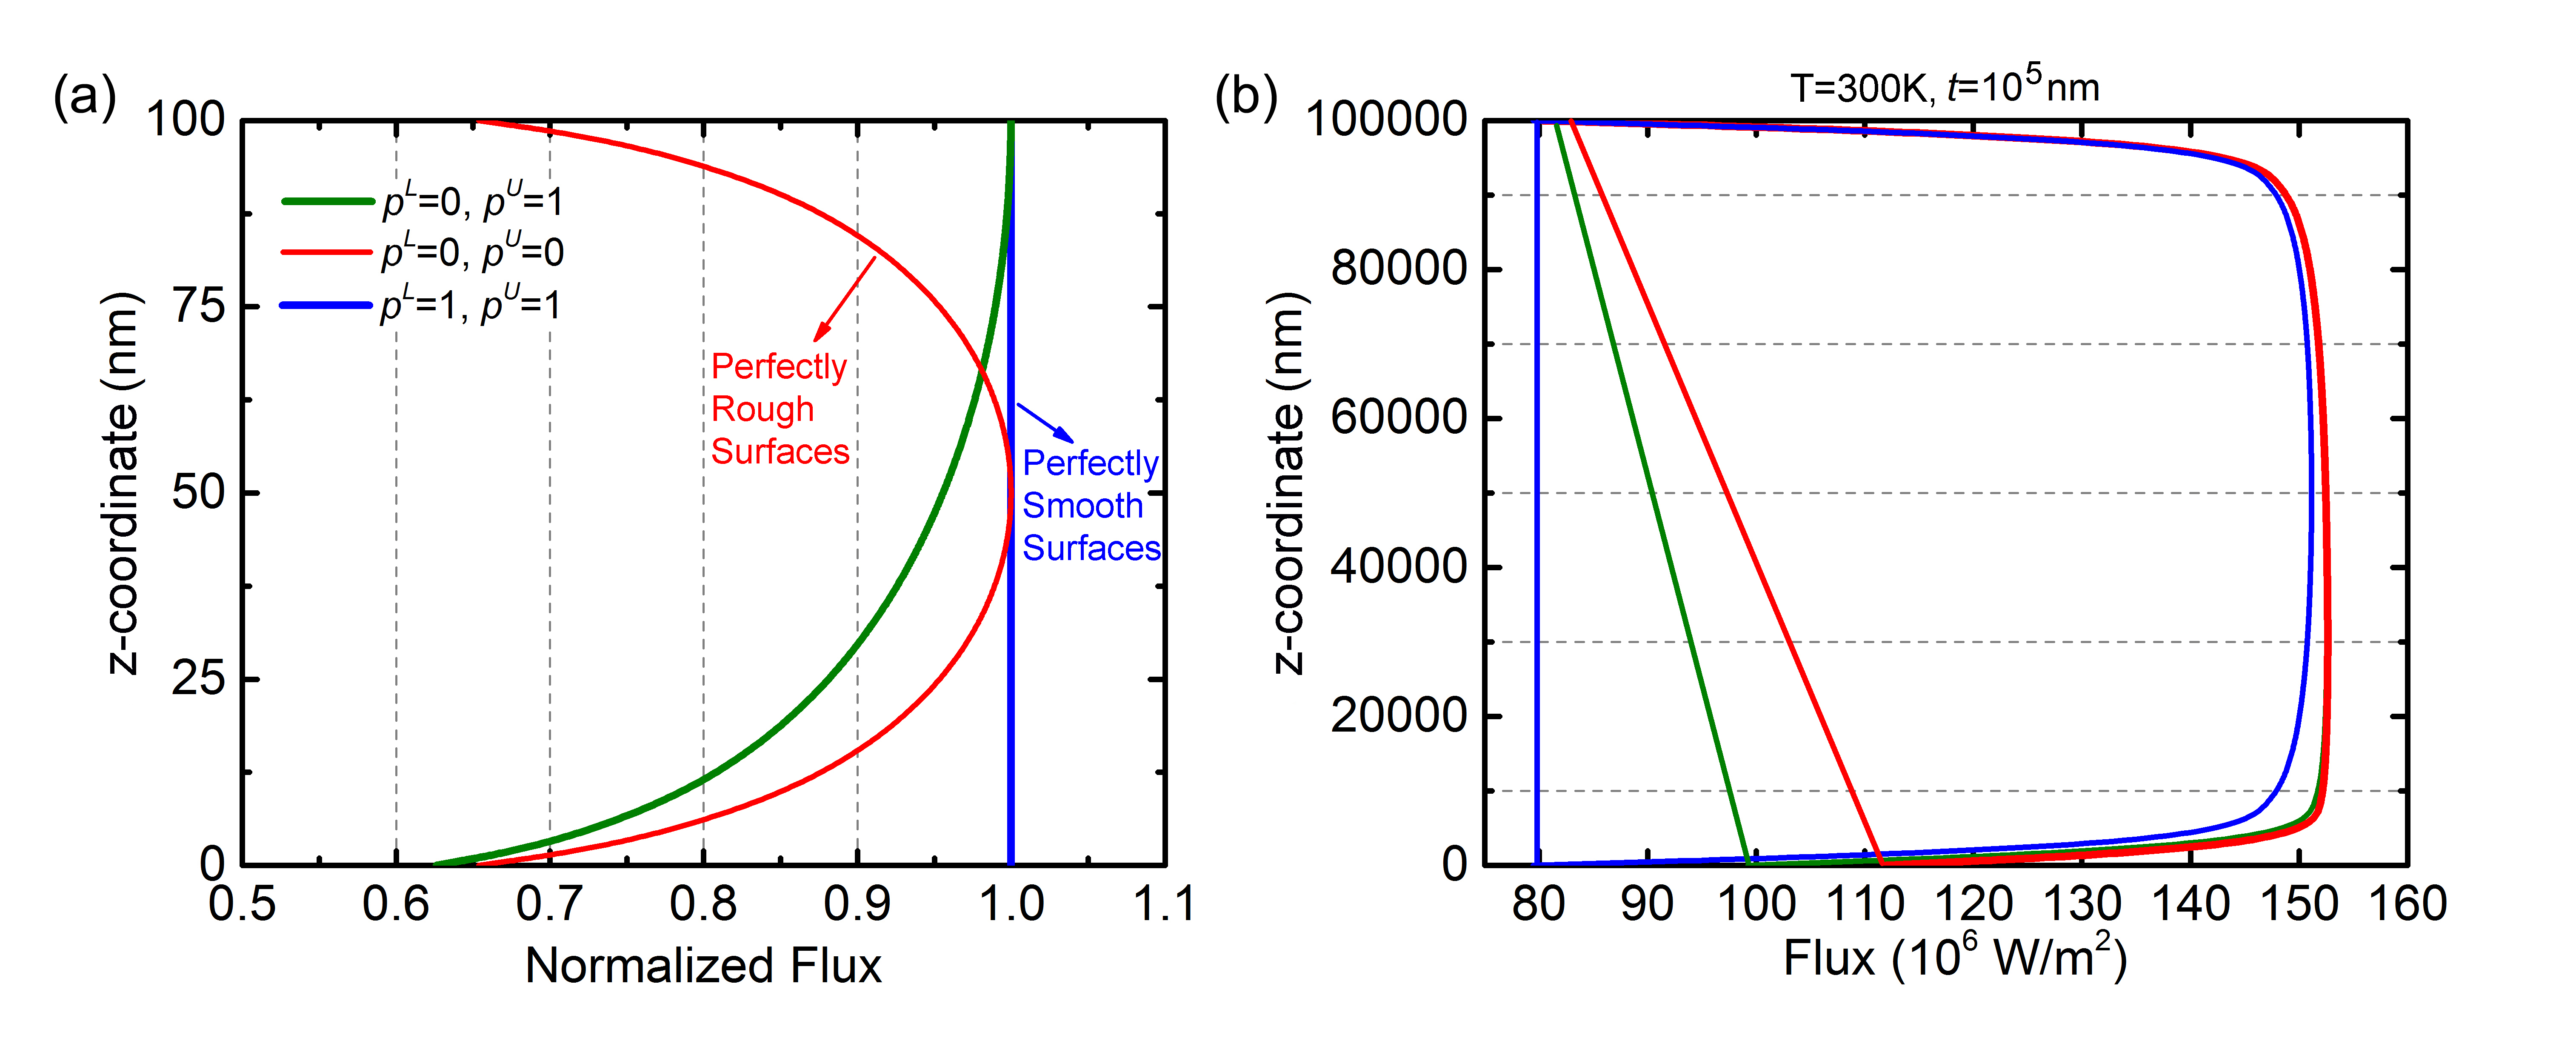
\includegraphics[width=1.0\textwidth]{figures/ch6/Fig5.jpg}
  \caption{Cross-plane thermal conductivity at \gls{T} = 300 K as a function of total superlattice size \gls{slsize} for [(a) and (b)] large periods \gls{period} = 50 nm and 200 nm, and [(c) and (d)] short periods \gls{period} = 4 nm and 10 nm. The solid lines represent smooth interfacial roughness \gls{eta} = 0.1 nm, and the dashed lines represent surface roughness \gls{eta} = 0.5 nm.}
  \label{fig:ch6-5}
\end{figure}
%Figure6
\begin{figure}[hbt]
  \centering 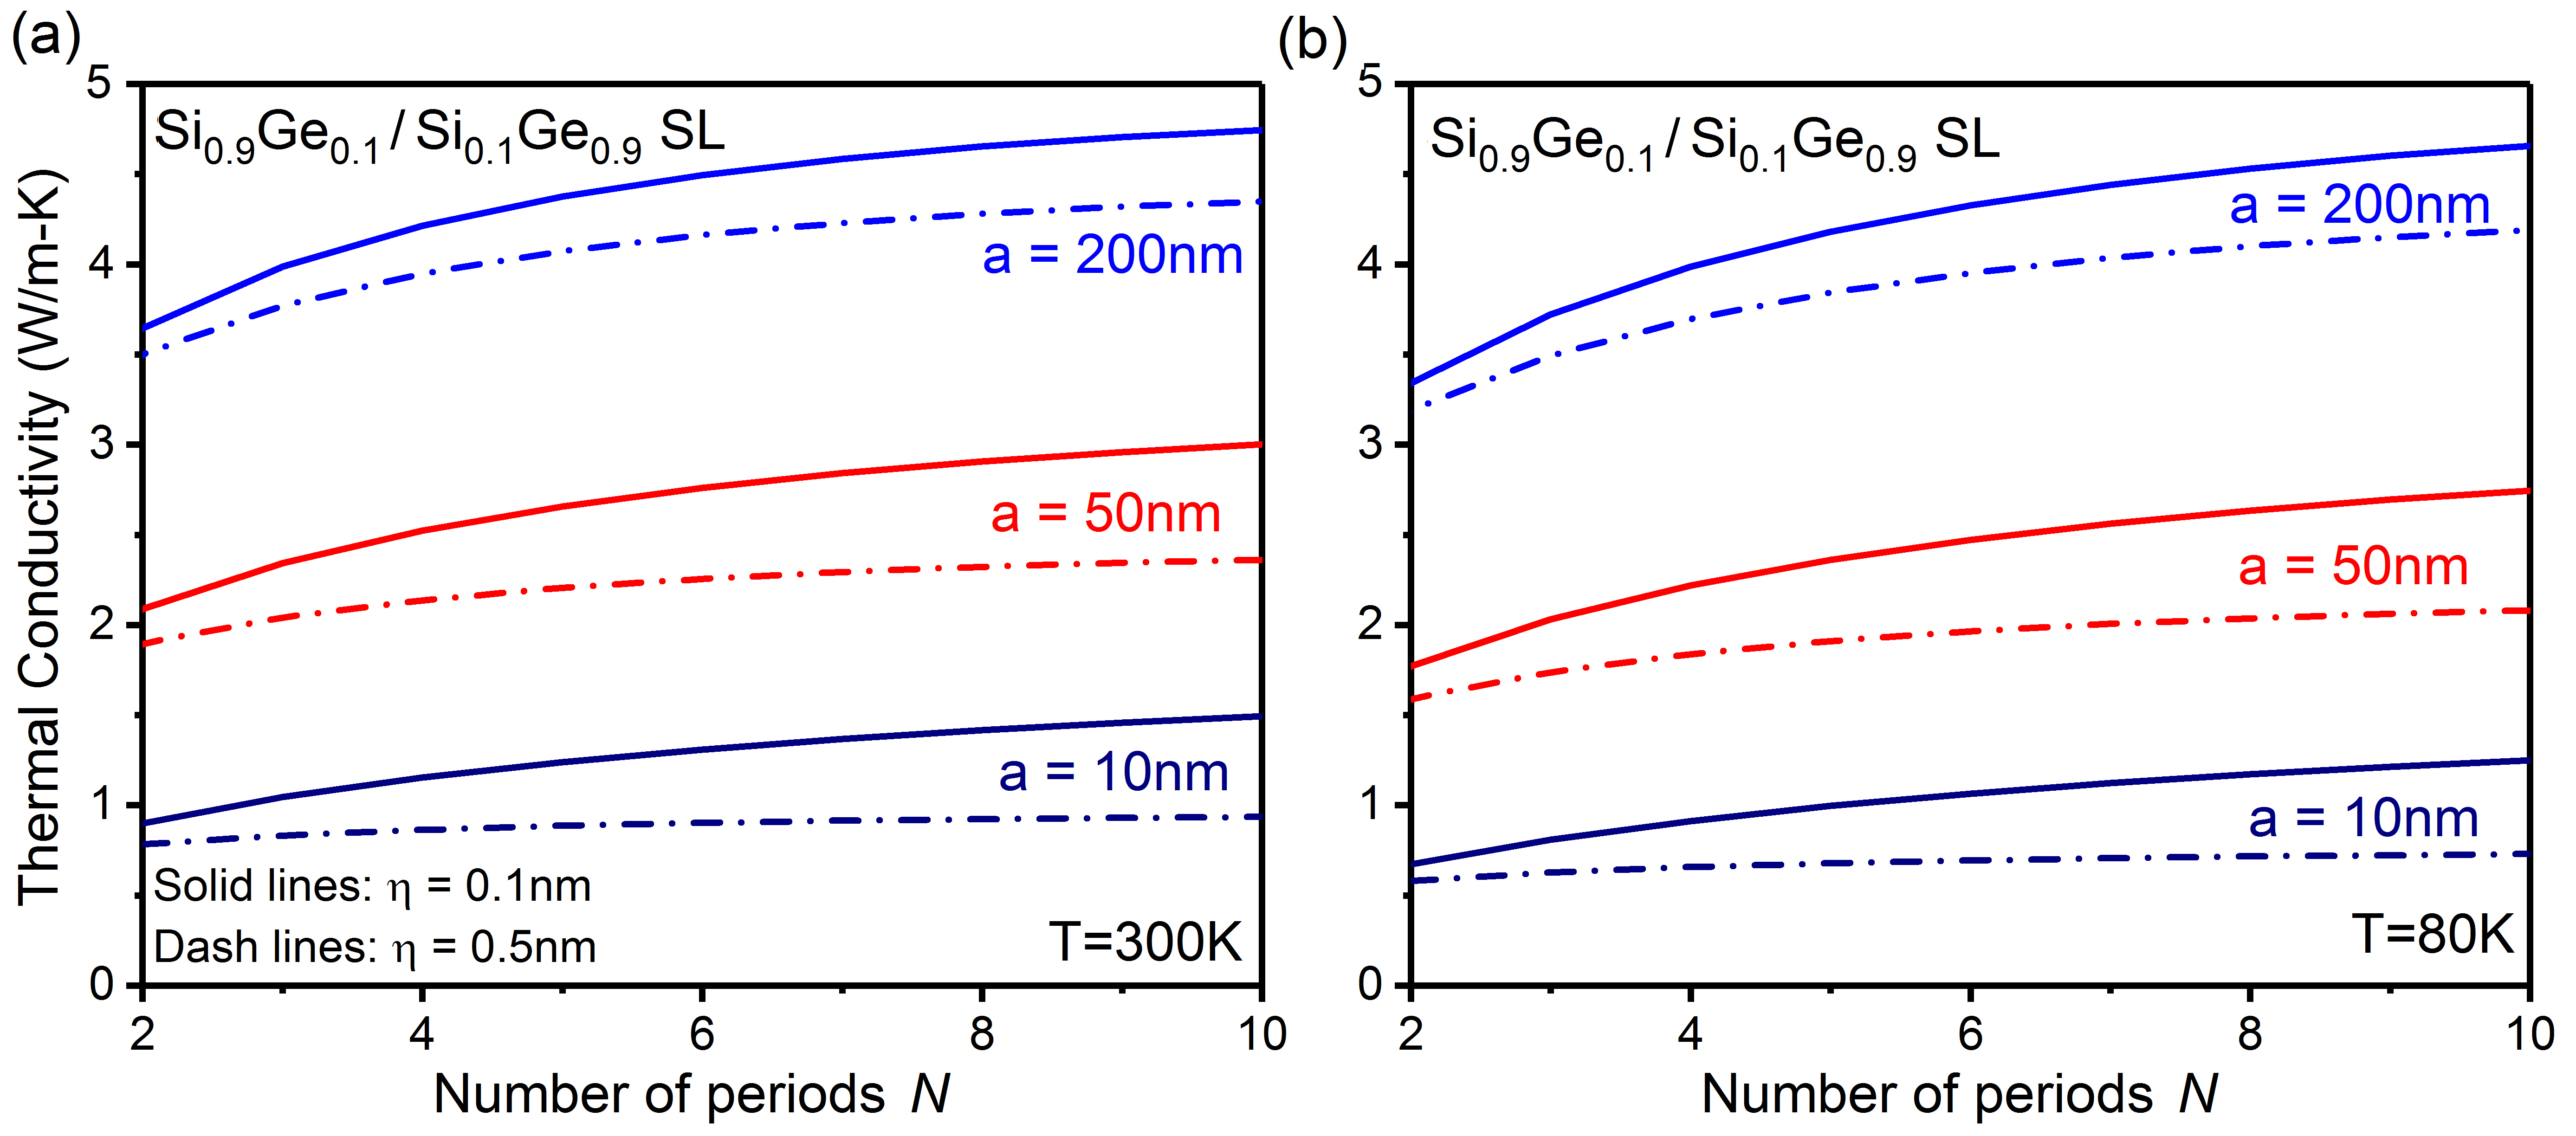
\includegraphics[width=1.0\textwidth]{figures/ch6/Fig6.jpg}
  \caption{Cross-plane thermal conductivity in alloyed superlattices at (a) \gls{T} = 300 K and (b) \gls{T} = 80 K as the function of number of periods $N$ in the superlattice. Three different periods \gls{period} = 10 nm (dark blue), 50 nm (red), and 200 nm (blue) are shown for two different surface conditions.}
  \label{fig:ch6-6}
\end{figure}
%Figure7
\par The layered structure of superlattices creates an anisotropic resistance to heat flow, providing a difference in thermal conductivities in the directions parallel and perpendicular to the interfaces. It is expected that when the thermal gradient is applied parallel to the interfaces (in-plane transport), phonon transport processes face less resistance from the boundaries than when the gradient is applied perpendicular to the interfaces \cite{book_Ziman}. This anisotropy in thermal transport is of great practical interest to create solid-state heat spreaders to better manage heat in electronic devices. We calculate the anisotropy in heat transport at 300 K (red lines) and 80 K (blue lines) in Si/Ge superlattices (\Cref{fig:ch6-7}) for different periods and interfacial conditions. We find that the anisotropy, defined as the ratio of in-plane to cross-plane thermal conductivity, reduces with increasing period \gls{period}. This indicates that with reduced interface density, both in-plane and cross-plane transport converge to the corresponding bulk values. For large roughness values, the diffusive scattering of phonons reduces the anisotropy ratio due to nearly saturated reduction in cross-plane conductivity. In contrast, for a given roughness, the anisotropy at \gls{T} = 80 K is larger than room temperature because at lower temperatures, resistance by phonon-phonon processes is diminished, allowing for the boundary scattering to dominate, which are stronger in the cross-plane direction. Based on the anisotropic thermal conductivities obtained for superlattices, it is clear that the cross-plane direction boundary scattering phenomenon is generally stronger compared to the in-plane direction. To further explore the transport of phonons in the two different directions, we evaluate their thermal spectra, i.e., the contribution of phonons of different wavelengths and mean-free-paths to total thermal transport. The conduction of heat by phonons with different wavelengths (or frequencies) and mean-free-paths is central to nanoscale thermal conduction. Normalized accumulation functions or heat-spectra have been utilized to understand nanoscale thermal transport in other nanostructures \cite{ownNW,RN236}.
\begin{figure}[hbt]
  \centering 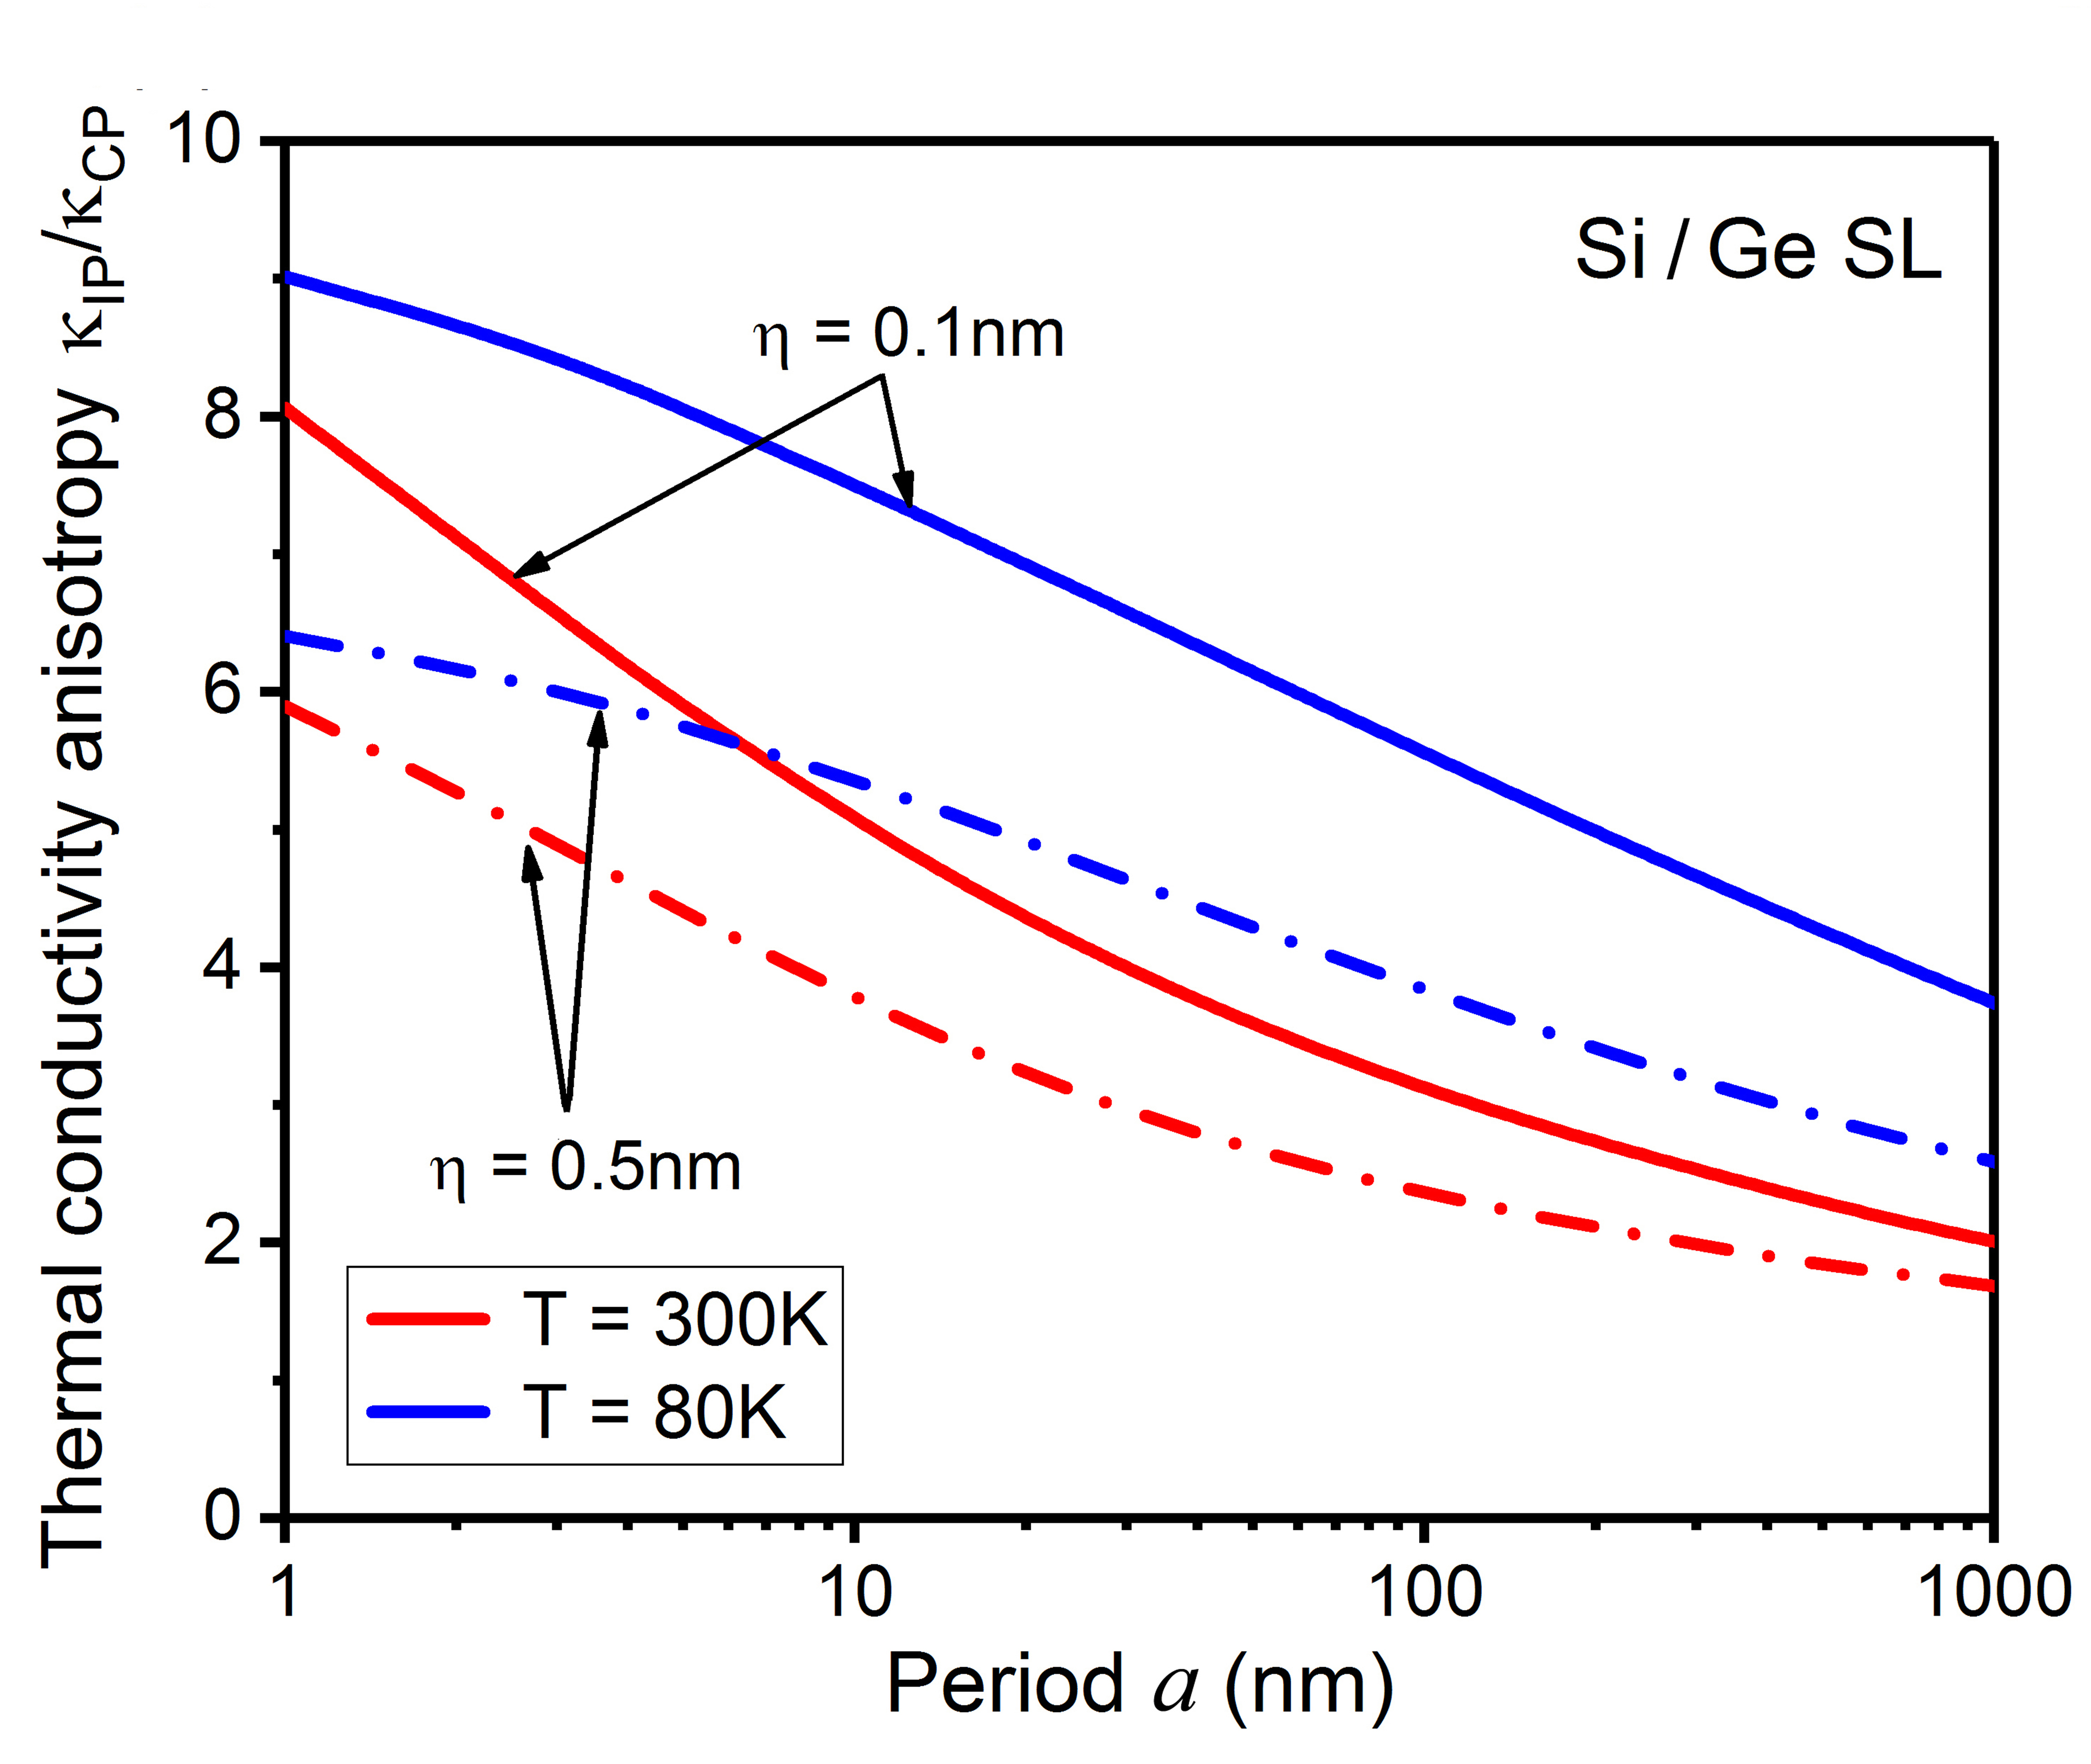
\includegraphics[width=0.80\textwidth]{figures/ch6/Fig7.jpg}
  \caption{The evolution of anisotropy in thermal conductivity with period thickness \gls{period} and roughness \gls{eta} in Si/Ge superlattices at room temperature (red lines) and \gls{T} = 80 K (blue lines).}
  \label{fig:ch6-7}
\end{figure}

%Figure8
\par However, cross-plane thermal transport in superlattices has not received similar attention. Using our developed methodology, we show our predictions for the cross-plane thermal heat spectra as a function of phonon wavelength at room temperature in \Cref{fig:ch6-8}(a,b), and compare it against the in-plane wavelength spectra in \Cref{fig:ch6-8}(c,d) \cite{RN396}. The increased surface scattering of large wavelength phonons caused by rougher interfaces (dashed lines) in all the cases (i.e., in-plane and cross-plane) shifts the thermal spectra to phonons of smaller wavelengths. Furthermore, surface scattering effects are stronger for shorter period superlattices owing to a higher interface density. However, in comparing between cross-plane and in-plane thermal spectra, we observe that the heat conduction in the cross-plane direction is shifted more strongly toward short-wavelength phonons reaffirming the understanding of enhanced surface effects when the gradient is applied perpendicular to interfaces. The difference between cross-plane and in-plane thermal spectra is observed even more clearly for alloyed superlattices. For the cross-plane SiGe alloy superlattice thermal transport [\Cref{fig:ch6-8}(b)], spectra are strongly suppressed such that phonons of wavelength \gls{wl} = 1–10 nm carry nearly all the heat. However, for the in-plane thermal transport, large wavelength phonons (\gls{wl} \textgreater 10 nm) contribute almost 35\% to heat transport for \gls{period} = 50 nm superlattices [\Cref{fig:ch6-8}(d)]. These findings clearly show that in cross-plane superlattice transport, the effects of surface scattering are stronger than in the in-plane direction. In particular, in cross-plane transport, phonons of wavelengths larger than \gls{wl} = 10 nm play no part in thermal transport at room temperature as they are effectively scattered out by scatterings at interfaces.
\begin{figure}[hbtp]
  \centering \includegraphics[width=1.0\textwidth]{figures/ch6/Fig8.jpg}
  \caption{Room temperature wavelength heat spectra for [(a) and (b)] cross-plane and [(c) and (d)] in-plane thermal transport in Si/Ge and \sige{0.90}{0.10}/\sige{0.10}{0.90} superlattices. Two different periods \gls{period} = 10 nm and \gls{period} = 50 nm and roughness values \gls{eta} = 0.1 nm and \gls{eta} = 0.5 nm are considered.}
  \label{fig:ch6-8}
\end{figure}

%Figure9
\par To understand the impact of surfaces on the mean-free-path spectra in superlattices, we consider periods \gls{period} = 50 nm (red lines) and \gls{period} = 10 nm (black lines), as well as surface roughnesses \gls{eta} = 0.1 nm and \gls{eta} = 0.5 nm in \Cref{fig:ch6-9}. We observe that with reducing period length and increasing roughness the heat spectra are shifted to smaller dominant mean-free-paths. This shift can be explained by a stronger interfacial scattering phenomenon in superlattices with smaller periods owing to their higher interfacial density and due to increased diffuse scattering with increasing surface roughness (dashed lines). Our predictions show that in the cross-plane direction heat flow in superlattices of up to period \gls{period} = 50 nm at room temperatures is controlled by phonons in the range of \gls{mfp} = 1–1000 nm. Even in alloyed superlattices where short mean-free-path phonons are scattered out of transport process, the thermal transport is upper bounded by \gls{mfp} = 1000 nm mean-free-path phonons, highlighting the strong role of interfacial scattering in the cross-plane direction. Since the surface properties can strongly influence the thermal transport in the cross-plane direction, quantification of experimental samples and better growth techniques would be the key drivers of future research in these superlattices.
\begin{figure}[hbt]
  \centering 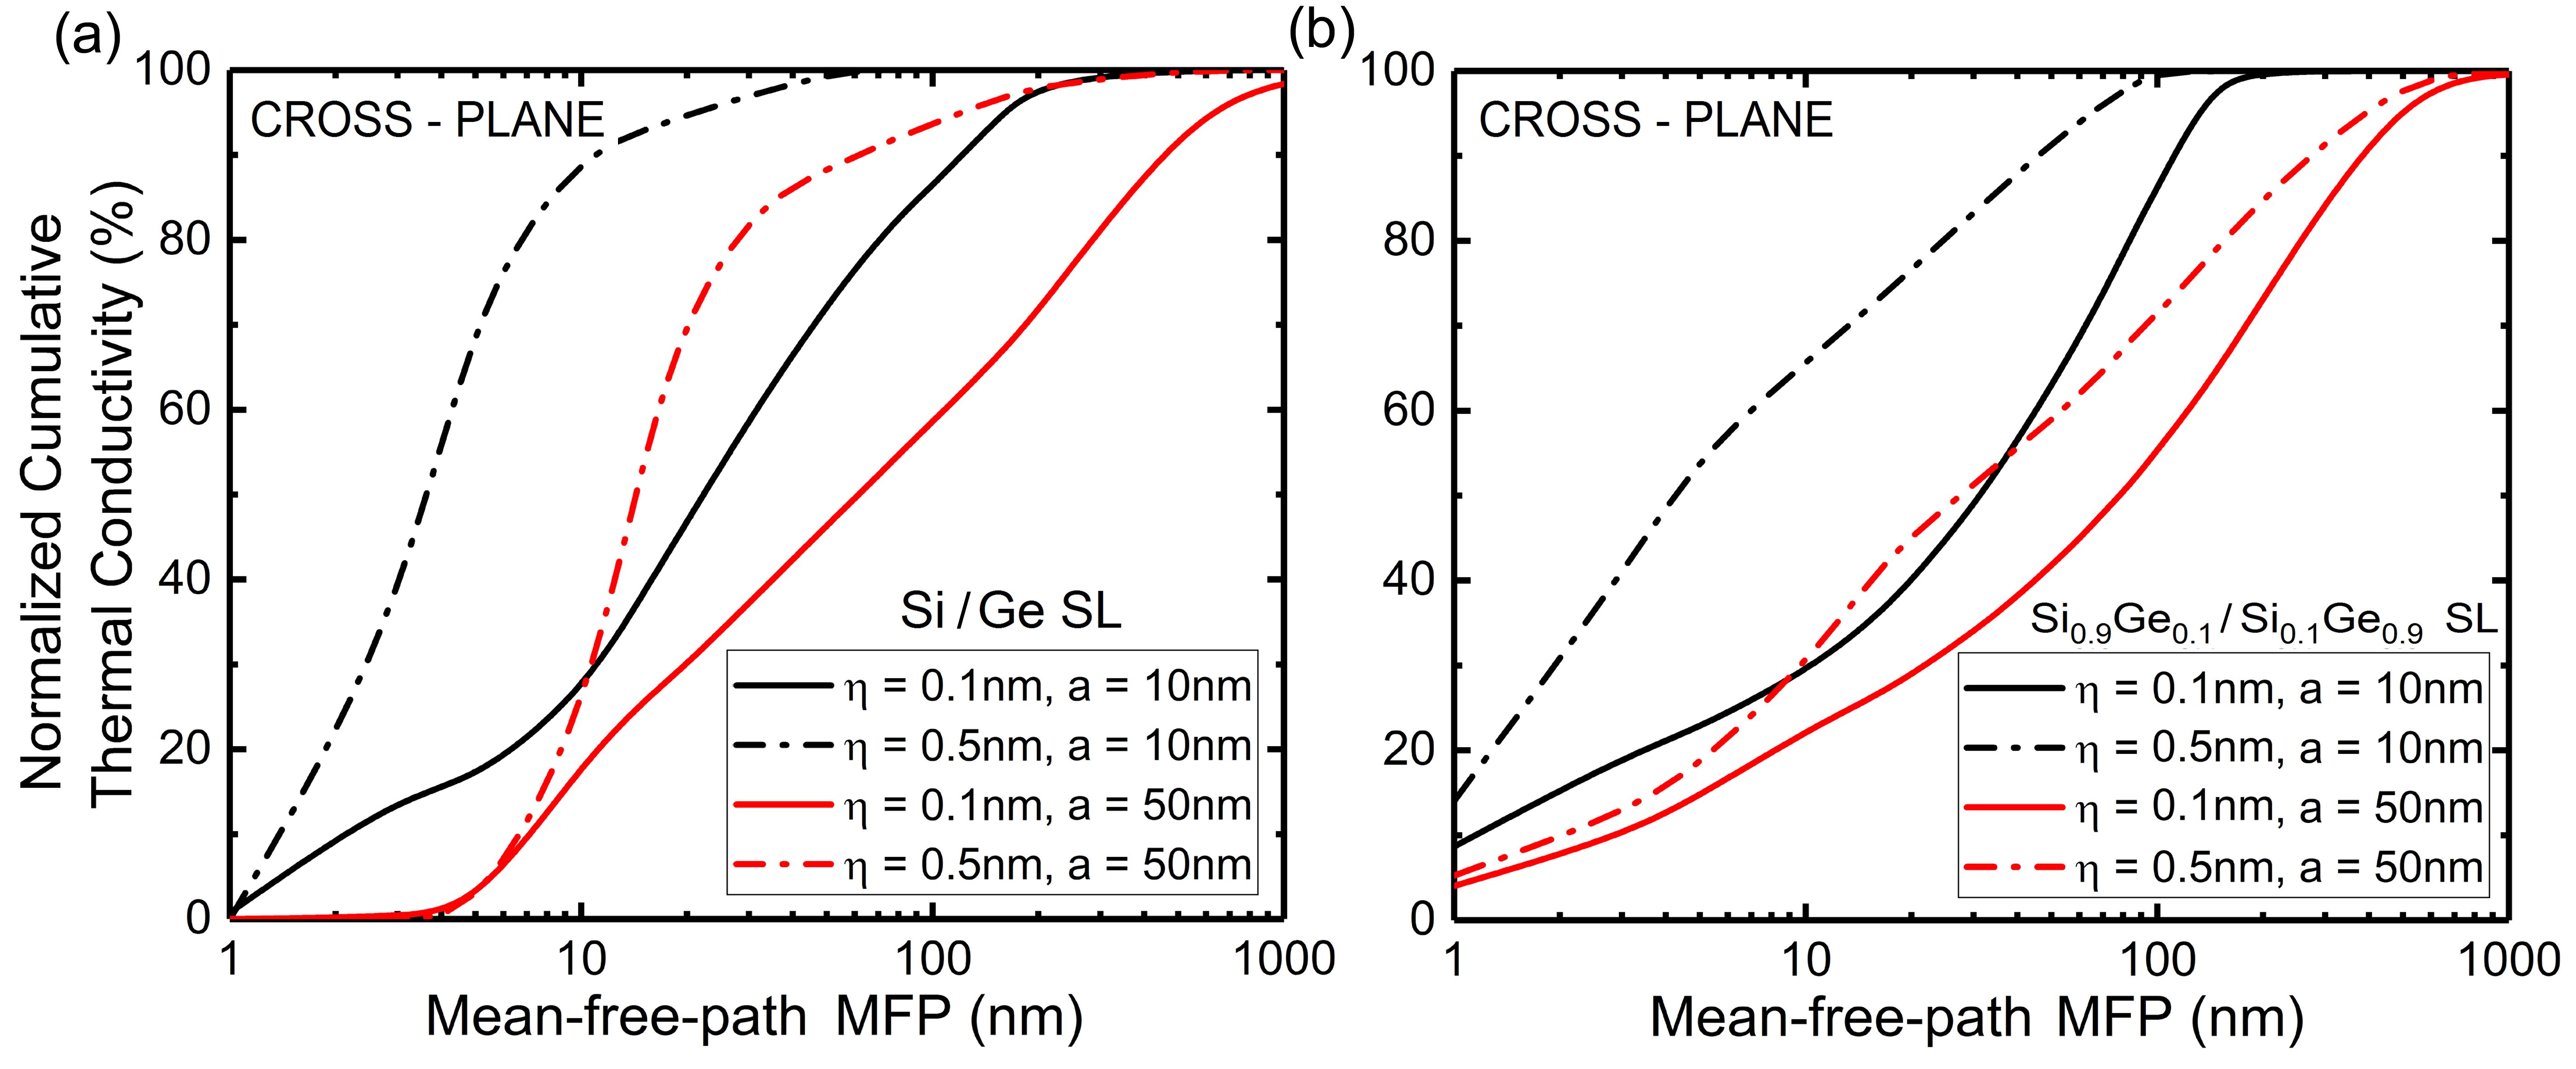
\includegraphics[width=1.0\textwidth]{figures/ch6/Fig9.jpg}
  \caption{Cross-plane thermal conductivity spectra at \gls{T} = 300 K as a function of phonon mean-free-path for superlattices of period 50 nm (red lines) and 10 nm (black lines) for smooth and rough interfaces in (a) Si/Ge and (b) \sige{0.90}{0.10}/\sige{0.10}{0.90} superlattices.}
  \label{fig:ch6-9}
\end{figure}

\section{Summary}
In this chapter, we extended the methodology developed in \Cref{chap:layered} to quantitatively predict and fundamentally understand incoherent cross-plane thermal transport in superlattices. We used our developed approach to study Si/Ge and SiGe alloyed superlattices in order to understand the role of all relevant length scales, i.e., interface roughness, period thickness, total structure thickness, phonon mean-free-path, and wavelength in the underlying thermal transport processes. Additionally, we unveiled the effects of alloying and temperature on cross-plane thermal transport in these superlattices. We found that thermal transport in cross-plane structures can be ballistic across the entire superlattice even at room temperatures. In addition, the contribution of large wavelength phonons is significantly suppressed in contrast to in-plane thermal transport, constraining the wavelength spectrum to less than 10 nm. These findings are essential toward efforts to rationally manipulating phonon transport and for future design of thermal transport processes in superlattices.


